\documentclass{article}

% Set page size and margins
% Replace `letterpaper' with `a4paper' for UK/EU standard size
\usepackage[letterpaper,top=2cm,bottom=2cm,left=3cm,right=3cm,marginparwidth=1.75cm]{geometry}

% Useful packages
\usepackage{ctex}
\usepackage{amsmath}
\usepackage{graphicx}
\usepackage{subfig}
\usepackage[colorlinks=true, allcolors=blue]{hyperref}
\usepackage{booktabs}
\usepackage{caption}
\usepackage[dvipsnames]{xcolor} % 更全的色系

\usepackage{listings} % 排代码用的宏包
%%%%%%%% listings设置 %%%%%%%%
\lstset{
	language = matlab,
	backgroundcolor = \color{yellow!10}, % 背景色:淡黄
	basicstyle = \small\ttfamily, % 基本样式 + 小号字体
	rulesepcolor= \color{gray}, % 代码块边框颜色
	breaklines = true, % 代码过长则换行
	numbers = left, % 行号在左侧显示
	numberstyle = \small, % 行号字体
	keywordstyle = \color{blue}, % 关键字颜色
%	commentstyle =\color{green!100}, % 注释颜色
	commentstyle =\color{purple!100}, % 注释颜色
	stringstyle = \color{red!100}, % 字符串颜色
	frame = shadowbox, % 用(带影子效果)方框框住代码块
	showspaces = false, % 不显示空格
	columns = fixed, % 字间距固定
	%escapeinside={} % 特殊自定分隔符:
	morekeywords = {as}, % 自加新的关键字(必须前后都是空格)
	deletendkeywords = {compile} % 删除内定关键字;删除错误标记的关键字用deletekeywords删!
}


%%%%%%%%% 页眉 %%%%%%%%%%%%
\usepackage{fancyhdr}
\pagestyle{fancy}
\lhead{}
\chead{《智能控制》神经网络控制作业}
\rhead{}

%%%%%%%%% 标题 %%%%%%%%%%%%
\title{《智能控制》神经网络控制作业}
\author{高瑞岚\quad 3190103249}
\date{}

%%%%%%%%%%% 正式文档 %%%%%%%%%%%%%
\begin{document}
\maketitle
\tableofcontents

%======================================
\section{BP神经网络系统辨识}
对真实系统模型
\begin{equation*}
    y(k+1) = \frac{y(k)-y(k-1)}{\sqrt{1+{y(k)}^2}}
    + {u(k)}^3
\end{equation*}
应用 BP 神经网络进行系统辨识。神经网络的输入向量为
\begin{equation*}
\mathbf{x} = 
\begin{bmatrix}
u(k) \\ y(k) \\ y(k-1)
\end{bmatrix}
\end{equation*}
输出为$ \mathbf{y} = y(k) $。
共采用2个隐层结构,其中第1个隐层包含20个神经元,第2个隐层包含10个神经元。

分别选择系统输入为$ u(k) = 0.5 \cos(6\pi k t_s) $
与$ u(k) = -0.75 \sin(12\pi k t_s) $,
样本点数为500与1000,比较结果如图 \ref{fig:bp} 所示。


\begin{figure}[htbp]
	\centering
	\subfloat[$ u(k) = 0.5 \cos(6\pi k t_s) $,样本点数为500]{
		\begin{minipage}{24em}
			\centering
			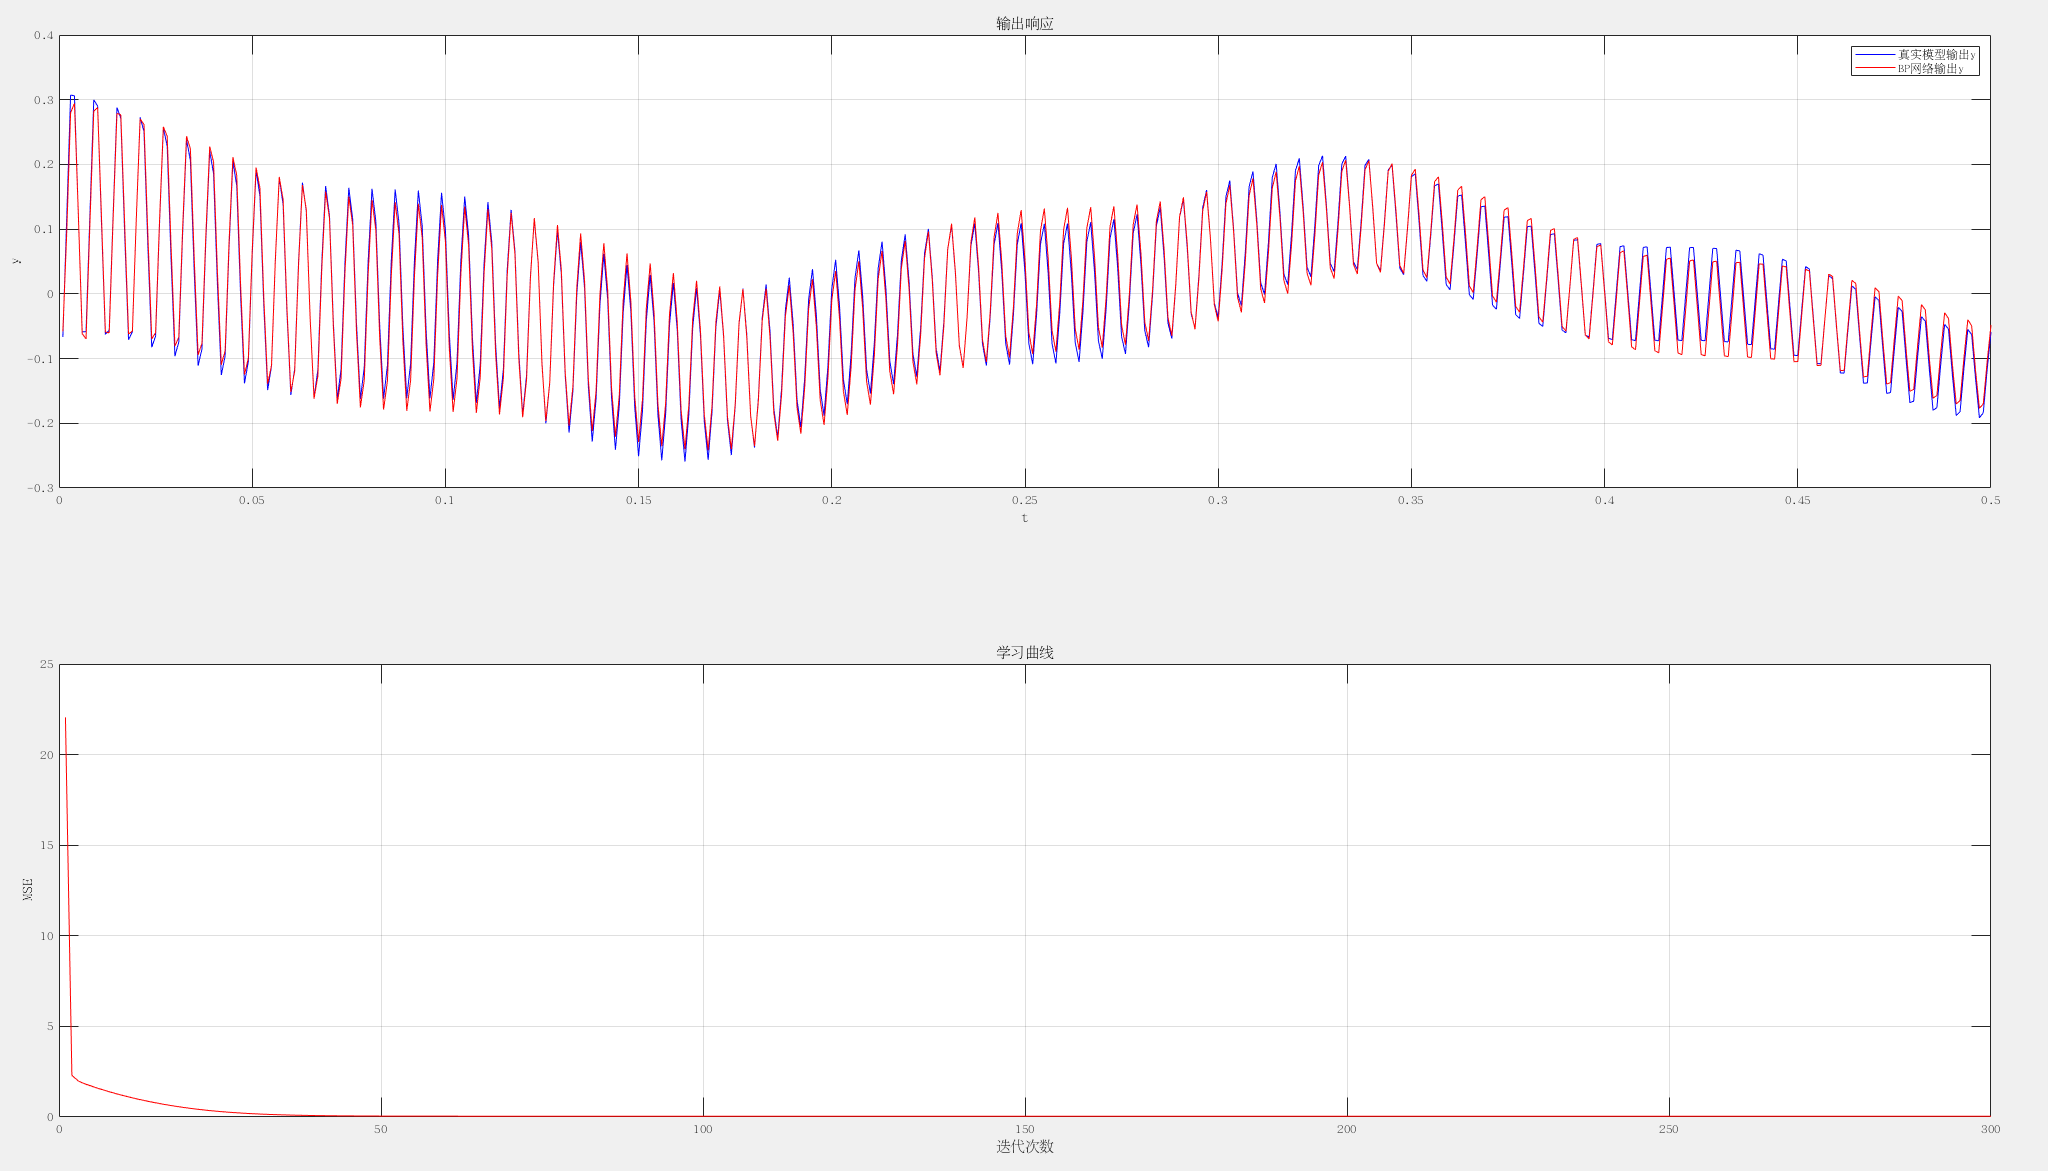
\includegraphics[width=1.0\textwidth]{pic/ex1/cos-500.png}
		\end{minipage}}
    
	\subfloat[$ u(k) = 0.5 \cos(6\pi k t_s) $,样本点数为1000]{
		\begin{minipage}{24em}
			\centering
			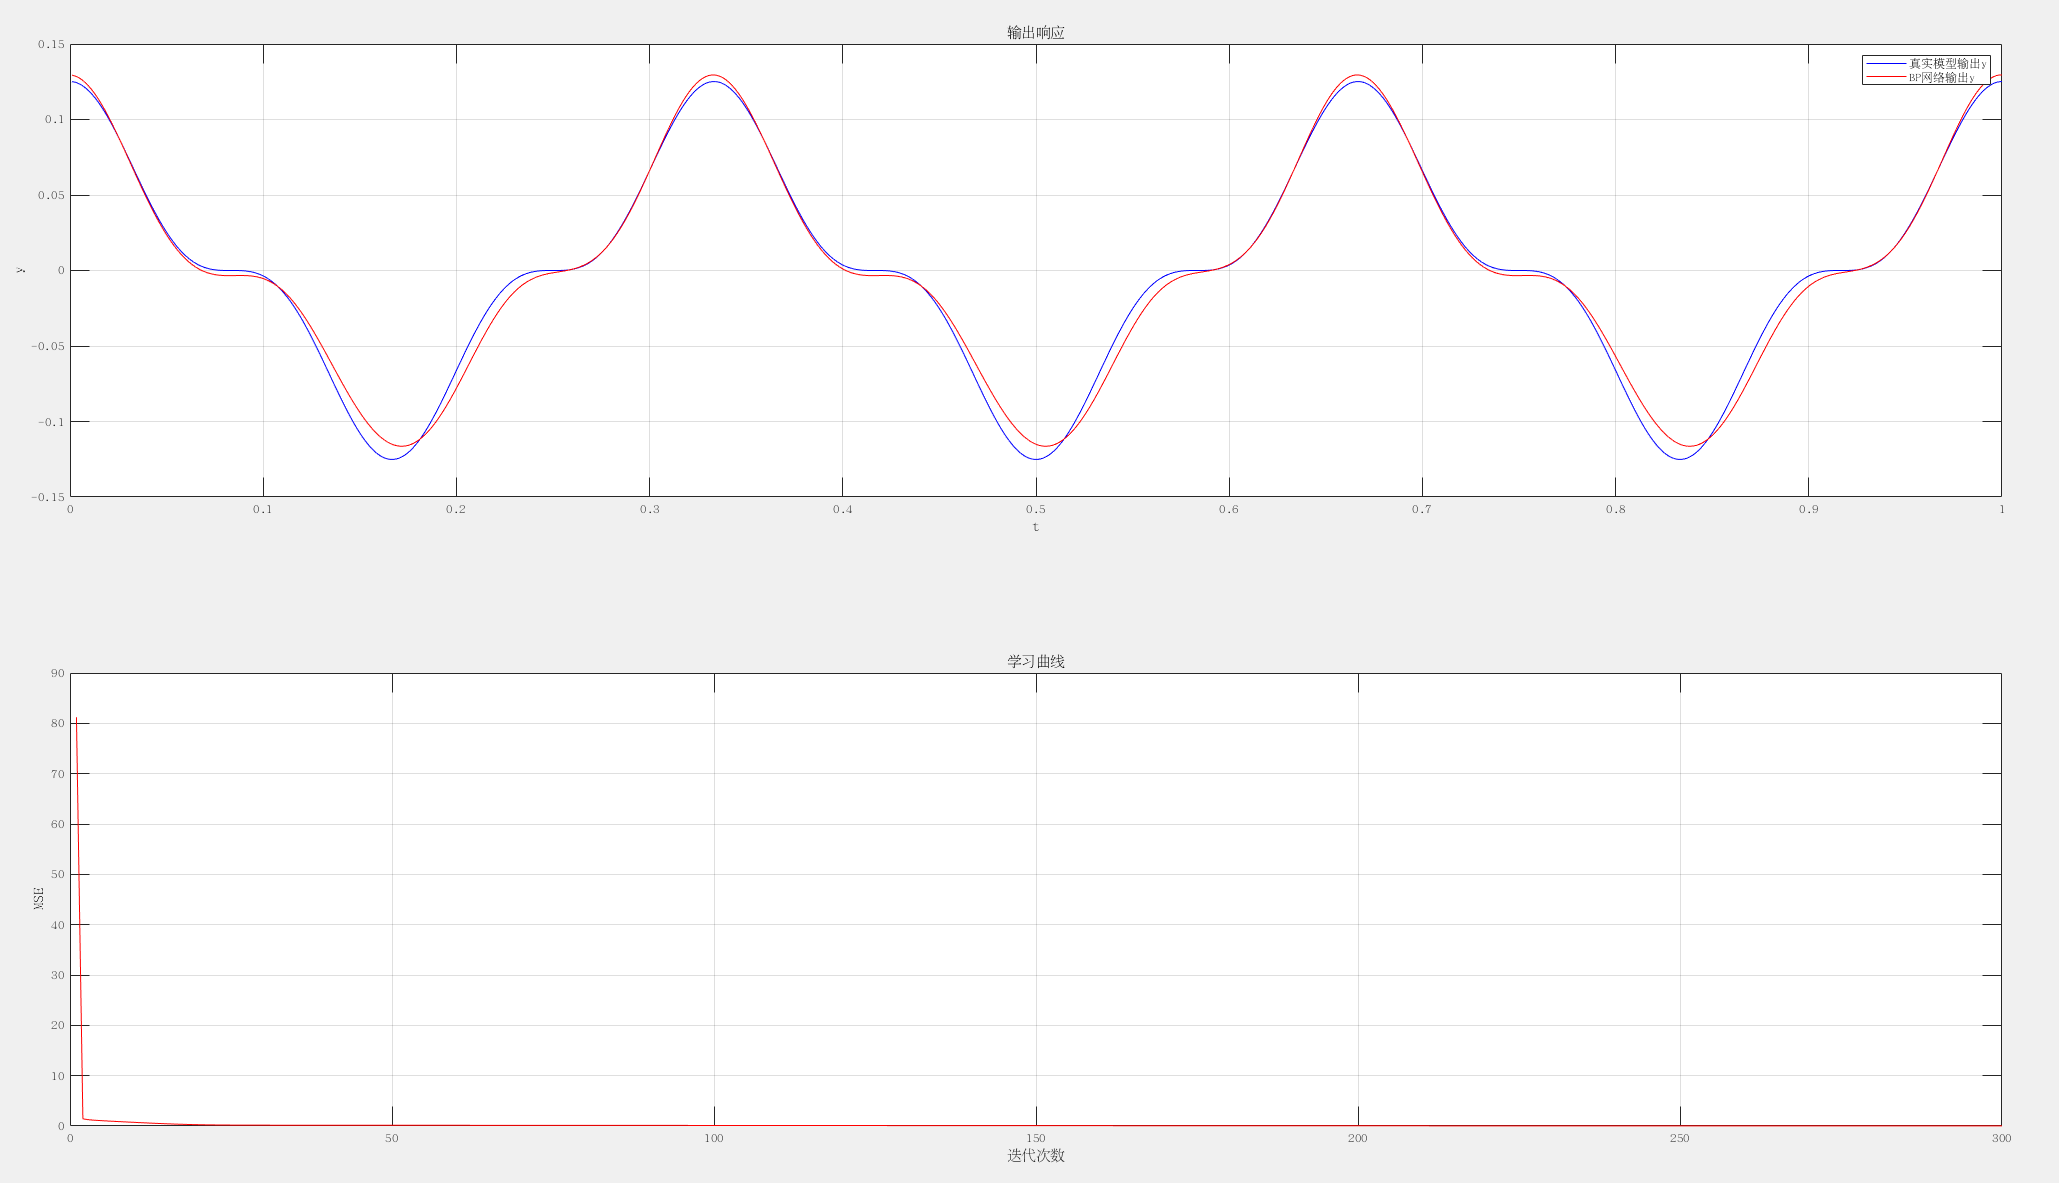
\includegraphics[width=1.0\textwidth]{pic/ex1/cos-1000.png}
		\end{minipage}}

	\subfloat[$ u(k) = -0.75 \sin(12\pi k t_s) $,样本点数为500]{
		\begin{minipage}{24em}
			\centering
			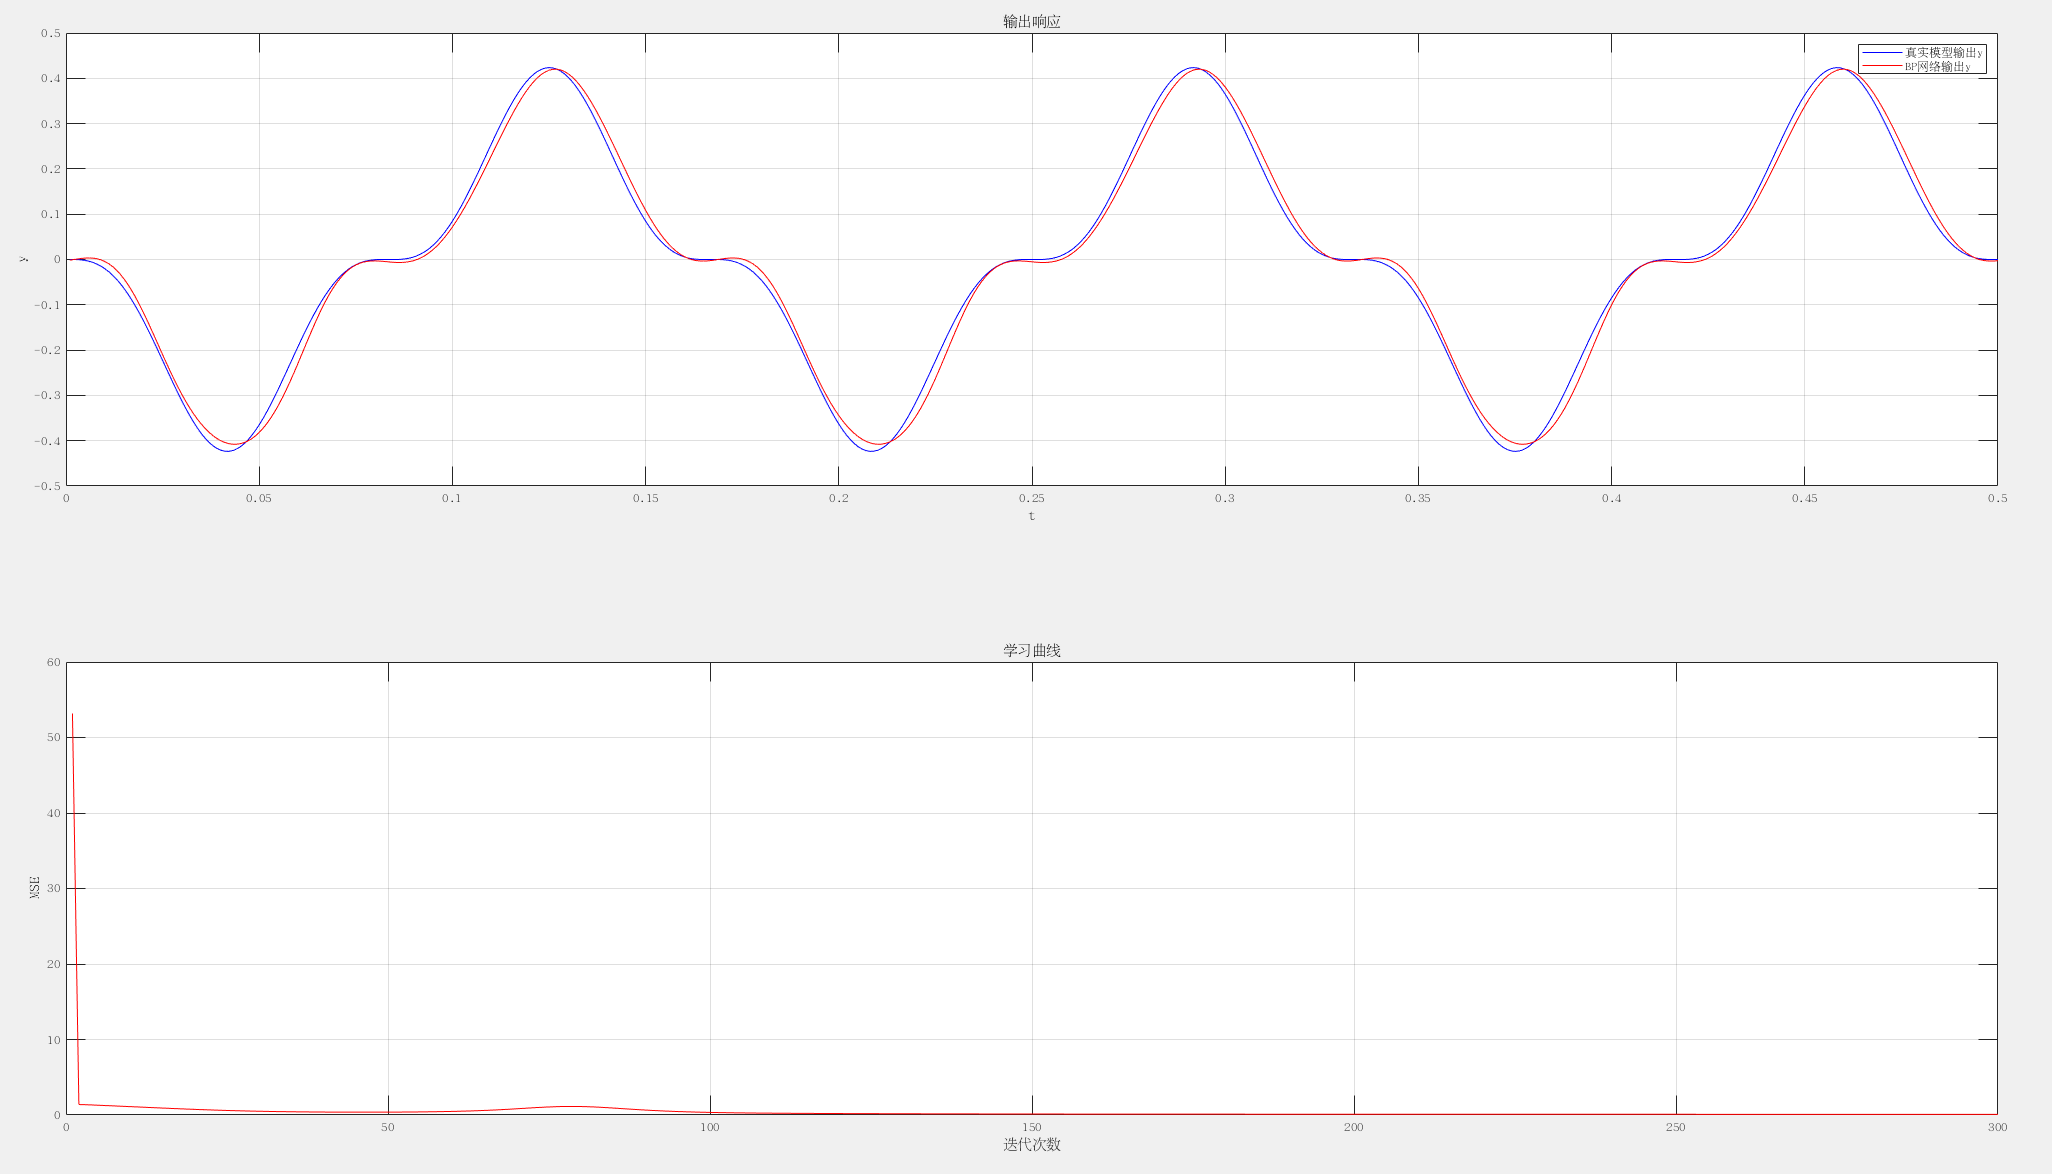
\includegraphics[width=1.0\textwidth]{pic/ex1/sin-500.png}
		\end{minipage}}
        
	\subfloat[$ u(k) = -0.75 \sin(12\pi k t_s) $,样本点数为1000]{
		\begin{minipage}{24em}
			\centering
			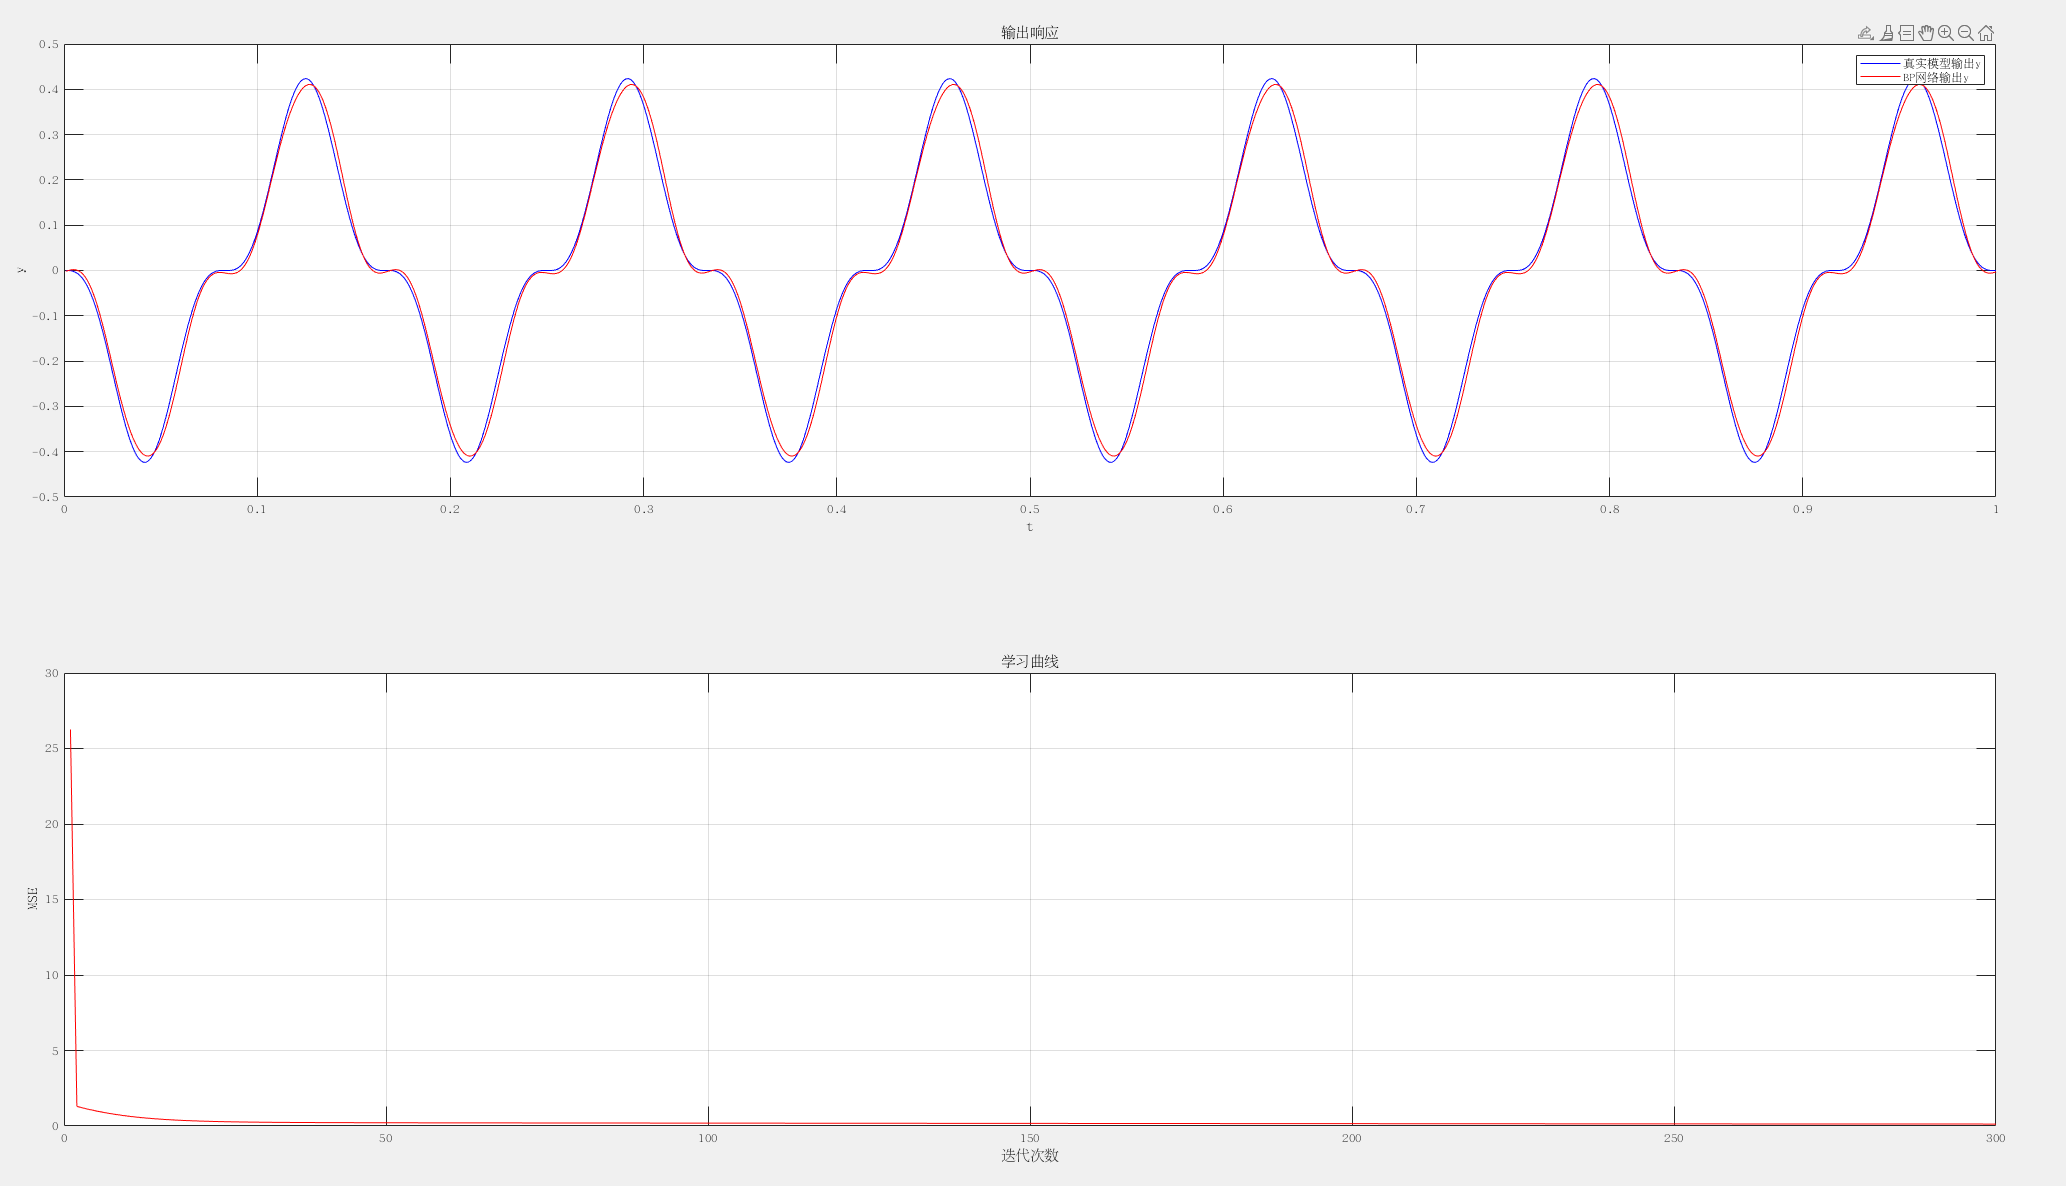
\includegraphics[width=1.0\textwidth]{pic/ex1/sin-1000.png}
		\end{minipage}}
	\caption{\label{fig:bp}BP神经网络系统辨结果比较}
\end{figure}



MATLAB程序如下所示。
\begin{lstlisting}[caption=ex1\_bp.m, language=matlab]
% ex1_bp.m
clc;clear;close all;

%% 参数初始化
l = 0.009;    % 学习率
alfa = 0.05;  % 动量因子

cells1 = 20;  % 隐层神经元个数
cells2 = 10;

w1 = rand(cells1,3);       % 随机赋值第一层连接权系数 [20  3]
w2 = rand(cells2,cells1);  % 随机赋值第二层连接权系数 [10  20]
w3 = rand(1,cells2);       % 随机赋值第三层连接权系数 [1   10]

yw1 = rand(cells1,1);  % 随机赋值第一层输出阈值 [20  1]
yw2 = rand(cells2,1);  % 随机赋值第二层输出阈值 [10  1]
yw3 = rand;            % 随机赋值第三层输出阈值 [1]

ts = 0.001;
%%%%%%%%%%%%%%%%%%%%%%%%%%
n = 500;  % 样本数
% n = 1000;  % 样本数
%%%%%%%%%%%%%%%%%%%%%%%%%%
yn = rand(1,n);  % 随机赋值输出(预测)
y  = rand(1,n);  % 随机赋值输出(真实)

counts = 1;  % 计数值初始化

x = [0,0,0]';  % 输入

u_1 = 0;  % 上一时刻的输入
y_1 = 0;  % 上一时刻的输出
y_2 = 0;  % 上上一时刻的输出

times = 300;  % 训练轮数
e = zeros(1,times);  % 均方差初始值设为0

%% 学习过程
for i = 1:times  % 学习轮数
    ei = 0;
    for a = 1:n  % 样本数
        time(a) = a*ts;
        
        %%%%%%%%%%%%%%%%%%%%%%%%%%
        % 系统输入
%         u(a) = 0.50*cos(6*pi*a*ts);
        u(a) = -0.75*sin(12*pi*a*ts);
        %%%%%%%%%%%%%%%%%%%%%%%%%%
        
        % 系统真实模型
        y(a) = (y_1 - y_2) / sqrt(1 + y_1^2) + u_1^3;
        
        net1 = w1*x - yw1;     % 第一层网络的输入 [20, 1]
        out1 = logsig(net1);   % 第一层网路的输出 [20, 1]
        net2 = w2*out1 - yw2;  % 第二层网络的输入 [10, 20]*[20 ,1]=[10, 1]
        out2 = logsig(net2);   % 第二层网络的输出 [10, 1]
        net3 = w3*out2 - yw3;  % 第三层网络的输出 [1]
        yn(a)= net3;           % 第三层网络的输出 [1]
        
        det3 = y(a) - yn(a);  % 计算偏差 [1]
        det2 = (det3 *w3) * out2 * (1-out2);  % ([1, 10]'*[10 ,1])*[10, 1] = [10, 1]
        det1 = (det2'*w2) * out1 * (1-out1); % [20, 1]
        
        w1 = w1 + det1*x'*l;       % [20, 2]
        w2 = w2 + (det2*out1')*l;  % [10, 20]
        w3 = w3 + (det3*out2')*l;  % [1, 10]
        
        yw1 = yw1 - det1*l;
        yw2 = yw2 - det2*l;
        yw3 = yw3 - det3*l;
        
        ei = ei + det3^2 / 2;
        e(i) = ei;
        
        % 更新输入
        x(1) = u(a);
        x(2) = y(a);
        x(3) = y_1;
        
        y_2 = y_1;
        u_1 = u(a);
        y_1 = y(a);
        
    end  % 结束一次样本遍历
    
    if ei < 0.008
        break;
    end
    counts = counts + 1;
end  % 结束学习

%% 绘图
figure(1);
subplot(2,1,1);
plot(time,y,'b-',time,yn,'r-');
legend('真实模型输出y', 'BP网络输出y')
grid on
title('输入u(k) = 0.50*cos(6*pi*k*ts)时的输出响应');
xlabel('t');
ylabel('y');

counts = counts - 1;
if (counts < times)
    count = 1:counts;
    sum = counts;
else
    count = 1:times;
    sum = times;
end

subplot(2,1,2);
plot(count,e(1:sum),'r-');
grid on;
title('学习曲线');
xlabel('迭代次数');
ylabel('MSE');

% END
\end{lstlisting}


%======================================
\section{神经网络控制器设计}




\end{document}
